\documentclass{article}
    % General document formatting
    \usepackage[margin=1in]{geometry}
    \usepackage[parfill]{parskip}
    \usepackage[utf8]{inputenc}
    \usepackage{amsmath,amssymb,amsfonts,amsthm}
    \usepackage{url}
    \usepackage{bm}
    \usepackage{graphicx}

\begin{document}

\title{A simple branching process model for Delta-variant and non-Delta-variant incidence of COVID-19 in Germany}
\author{Johannes Bracher}


\maketitle
\bigskip

\textit{This is just a sketch shared via a GitHub repository to facilitate discussion. While I think that the results are reasonable, please keep in mind that this is a rather simple model taking into account only the fact that there are two co-corculating variants. Vaccination, population behaviour, NPIs etc are ignored. Also, I set this up quite quickly and cannot guarantee that there are no technical mistakes.}

\section{Data and notation}

The model involves the following quantities:

\begin{itemize}
\item To describe the epidemic process:
\begin{itemize}
\item $X_t$: The total number of notified cases in week $t$, either from RKI or JHU (both by reporting date to the natinal authorities). Weeks run from Sunday through Saturday to ensure comparability to the Forecast Hub.
\item $X^\Delta_t, X^o_t$: The number of Delta and other cases among the notified cases, respectively (unobserved)
\item $r^\Delta_t, r^o_t$: One plus the weekly growth rate of the Delta variant and other variants combined, respectively.
\item $\psi^\Delta, \psi^o$: Overdispersion parameters for the two variants.
\item $\omega^\Delta_t, \omega^o_t$ auxiliary variables needed to express the negative binomial distributions as a Poisson-gamma mixture.
\item $\lambda^\Delta_t, \lambda^o_t$: Conditional expectations of $X^\Delta_t, X^o_t$ given $X^\Delta_{t - 1}, X^o_{t - 1}$ and $\omega^\Delta_t, \omega^o_t$.
\end{itemize}
\item To describe the sequencing:
\begin{itemize}
\item $N_t$: The number of sequenced cases in the random sample from RKI in week $t$. Note: These weeks are defined as Monday through Sunday.
\item $Y^\Delta_t$: The number among these which are from the Delta variant in week $t$.
\end{itemize}
\end{itemize}

\textbf{Caveat:} The definition of the weeks for the different data streams is not identical, and I am not sure whether one needs to shift one of them slightly to have them actually refer to the same time periods. The sequencing data are by date of sampling, while the incidence data are by date of reporting to the national authorities.

\section{Model formulation}

I apply a fully Bayesian model defined as follows. The total number of observed cases is decomposed into
$$
X_t = X^\Delta_t + X^o_t
$$
and assume negative binomial branching processes for $X^\Delta_t$ and $X^o_t$:
\begin{align*}
X^{(\cdot)}_t \ \mid \ \lambda^{(\cdot)}_t & \sim \text{Pois}(\lambda_t)\\
\lambda^{(\cdot)} & = \omega_t \times r_t \times X^{(\cdot)}_{t - 1}
\end{align*}
Here, $\omega^{(\cdot)}_t$ is an auxiliary gamma-distributed random variable,
$$
\omega^{(\cdot)}_t \sim \text{Gamma}(\psi^{(\cdot)}, \psi^{(\cdot)})
$$
meaning that without conditioning on $\omega^{(\cdot)}_t$ the $X^{(\cdot)}_t$ are negative binomial with mean $r^{(\cdot)}_t X^{(\cdot)}_{t - 1}$ and dispersion parameter $\psi^{(\cdot)}$. For the time-varying weekly multiplication factors $r^{(\cdot)}_t$ (one plus growth rate) we assume a random walk structure,
\begin{align*}
r^{(\cdot)}_t & = r^{(\cdot)}_{t - 1} \times \exp(\epsilon^{(\cdot)}_{t})\\
\epsilon^{(\cdot)} & \sim \text{N}(0, \sigma^{2(\cdot)}).
\end{align*}
We thus assume that the $r^{(\cdot)}_t$ show some smoothness and cannot change too quickly. \textbf{Caveat:} This formulation of the random walk is advantageous as it ensures that $r^{(\cdot)}_t$ is always positive. However, it may introduce a slight upward trend on the scale of $r^{(\cdot)}_{t}$ (as $\mathbb{E}(r^{(\cdot)}_{t + 1} \ \mid \ r^{(\cdot)}_{t}) > r^{(\cdot)}_{t}$). However, I am unsure how this translates to the case scale.

For the sequencing results we add the following observation process:
$$
Y^\Delta_t \ \mid \ N_t \sim \text{Bin}(N_t, p^\Delta_t),
$$
where
$$
p^\Delta_t = \frac{X^\Delta_t}{X_t}.
$$

To complete the model we need to specify some prior distributions for the parameters and initialization of the epidemic process:
\begin{align*}
1/\sigma^{2(\cdot)} & \sim \text{Unif}(5, 200)\\
\psi^{(\cdot)} & \sim \text{Unif}(0, 100)\\
X^\Delta_{16} & \sim \text{Unif}(0, 1000.)\\
\end{align*}
These are intended to be ``uninformative'', motivating priors for these parameters is not straightforward.

\section{Inference}

I generate samples from the posterior distribution of the various unobserved and predicted quantities using the \texttt{JAGS} software via the \texttt{R} package \texttt{runjags} (see \texttt{JAGS\_model.R} for the code). I generate 50,000 samples from 5 chains after a burn-in period of 4,000 samples.

\section{Results}

I ran the model on the RKI and JHU data and obtained the results shown in Figures 1 and 2. While the data imply slightly different current case levels, in both cases the extrapolation of trends implies a rather sudden flattening of the overall case counts which had previously been decaying steadily. The data which have accumulated since the last used data point point into this direction, too, even though the flattening may not be as abrupt as implied by the point predictions. Note that the model implies a lot of uncertainty and for more than one week ahead actually makes very uninformative predicitons. In three weeks the Delta variant will have become strongly dominant.

Note that the availability of sequencing results lags behind the available incidence data ad there is one week for which the overall case count is already known while the sequencing results are not. This is reflected by a widening of the uncertainty intervals for the strain-specific numbers.

\begin{figure}
\center
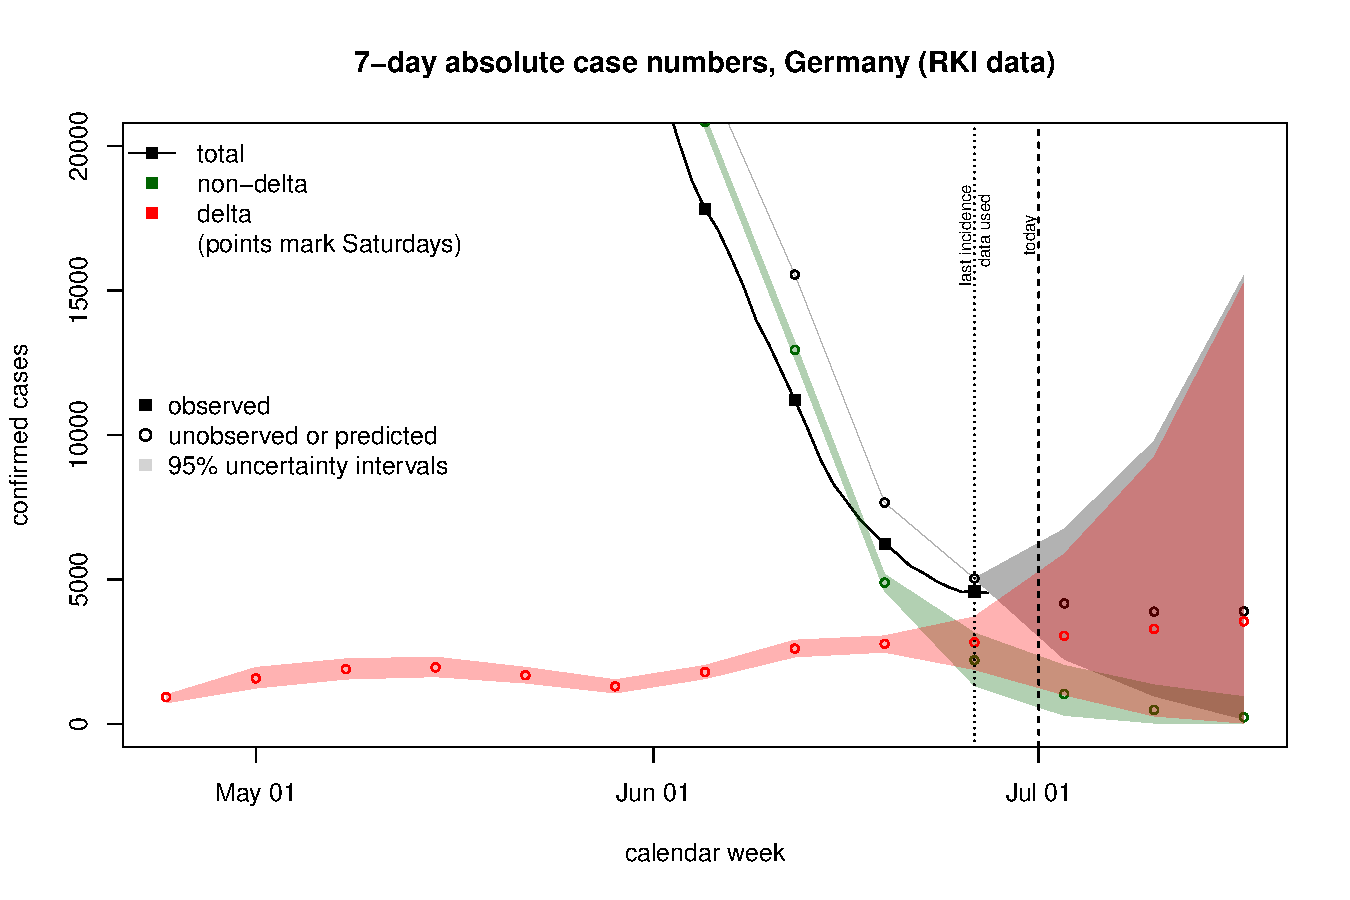
\includegraphics[scale=0.6]{plots/plot_RKI_2021-07-01.pdf}
\caption{Results based on RKI data, 1 July 2021.}
\end{figure}

\begin{figure}
\center
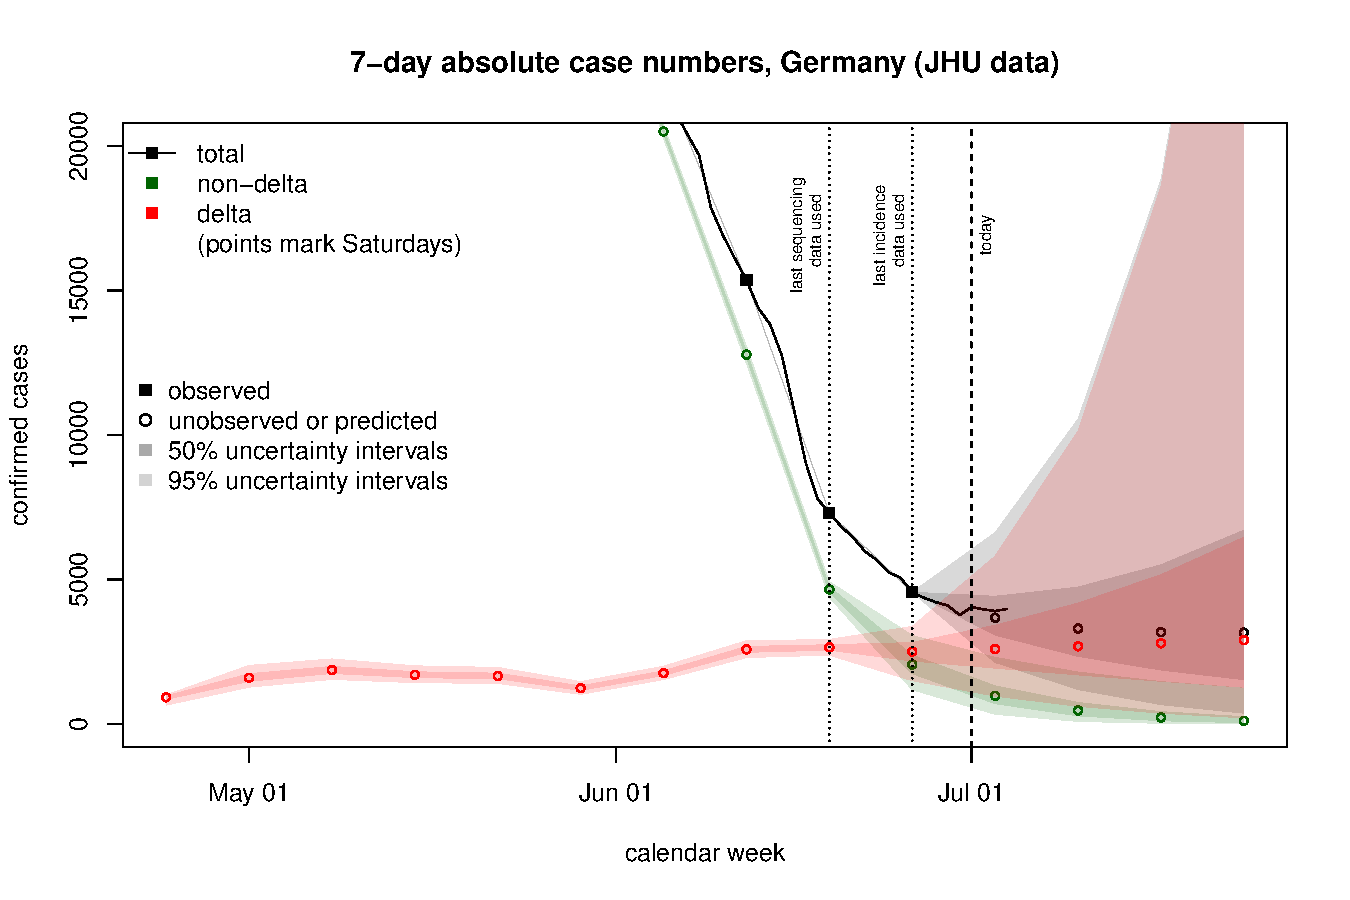
\includegraphics[scale=0.6]{plots/plot_JHU_2021-07-01.pdf}
\caption{Results based on JHU data, 1 July 2021.}
\end{figure}
\end{document}
